\begin{flushright} {\tiny {\color{gray} (tikz\_p4.tex)}} \end{flushright}
%~~~~~~~~~~~~~~~~~~~~~~~~~~~~~~~~~~~~~~~~~~~~~~~~~~~~~~~~~~~~~~~~~~~~~~~~~~~~~~~~~~~~~~~~~~~~~~~~~~

\begin{center}
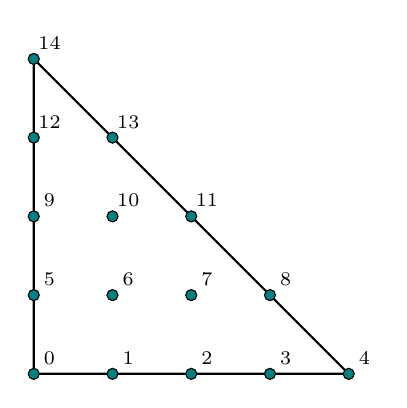
\begin{tikzpicture}
%\draw[step=0.5cm,gray,very thin] (0,0) grid (5,3.5); %bckgr grid
\draw[thick] (0,0) -- (4,0)  -- (0,4) -- cycle; 

\draw[black,fill=teal] (0,0) circle (2pt);
\draw[black,fill=teal] (1,0) circle (2pt);
\draw[black,fill=teal] (2,0) circle (2pt);
\draw[black,fill=teal] (3,0) circle (2pt);
\draw[black,fill=teal] (4,0) circle (2pt);
\draw[black,fill=teal] (0,1) circle (2pt);
\draw[black,fill=teal] (1,1) circle (2pt);
\draw[black,fill=teal] (2,1) circle (2pt);
\draw[black,fill=teal] (3,1) circle (2pt);
\draw[black,fill=teal] (0,2) circle (2pt);
\draw[black,fill=teal] (1,2) circle (2pt);
\draw[black,fill=teal] (2,2) circle (2pt);
\draw[black,fill=teal] (0,3) circle (2pt);
\draw[black,fill=teal] (1,3) circle (2pt);
\draw[black,fill=teal] (0,4) circle (2pt);

\node[] at (0.2,0.2) {\scriptsize $0$};
\node[] at (1.2,0.2) {\scriptsize $1$};
\node[] at (2.2,0.2) {\scriptsize $2$};
\node[] at (3.2,0.2) {\scriptsize $3$};
\node[] at (4.2,0.2) {\scriptsize $4$};
\node[] at (0.2,1.2) {\scriptsize $5$};
\node[] at (1.2,1.2) {\scriptsize $6$};
\node[] at (2.2,1.2) {\scriptsize $7$};
\node[] at (3.2,1.2) {\scriptsize $8$};
\node[] at (0.2,2.2) {\scriptsize $9$};
\node[] at (1.2,2.2) {\scriptsize $10$};
\node[] at (2.2,2.2) {\scriptsize $11$};
\node[] at (0.2,3.2) {\scriptsize $12$};
\node[] at (1.2,3.2) {\scriptsize $13$};
\node[] at (0.2,4.2) {\scriptsize $14$};

\end{tikzpicture}
\end{center}
